\documentclass[10pt]{article}
\usepackage[utf8]{inputenc}
\usepackage[T1]{fontenc}
\usepackage{amsmath}
\usepackage{amsfonts}
\usepackage{amssymb}
\usepackage[version=4]{mhchem}
\usepackage{stmaryrd}
\usepackage{graphicx}
\usepackage[export]{adjustbox}
\graphicspath{ {./images/} }

\begin{document}
\begin{enumerate}
  \item By calculating the limit
\end{enumerate}

$$
\lim _{h \rightarrow 0} \frac{f(x+h)-f(x)}{h}
$$

find the derivatives of the following functions at $x=a$ :\\
(a) $f(x)=\frac{1}{x}$ for $a \neq 0$.\\
(b) $f(x)=\sqrt{x}$ for $a \neq 0$.\\
(c) $f(x)=\frac{1}{\sqrt{x}}$ for $a \neq 0$.\\
(d) $f(x)=x^{3}-3 x+5$.\\
(e) $f(x)=x^{1 / 4}$.\\
(f) ${ }^{*} f(x)=\sin \left(x^{2}\right)$.\\[0pt]
[Hint: For (f) you can use that as $h$ approaches $0, \sin h \approx h$ and $\cos h \approx 1-h^{2}$ ]

\section*{GROUP WORK 1, SECTION 2.7}
Follow that Car\\
The distance travelled by a car is given by $d(t)=8\left(t^{3}-6 t^{2}+12 t\right)$, where $d$ is in miles and $t$ is in hours.

\begin{enumerate}
  \item Draw a graph of $d(t)$ from $t=0$ to $t=3$.
  \item Does the car ever stop?
  \item What is the average velocity over $[1,3]$ ? over $[1.5,2.5]$ ? over $[1.9,2.1]$ ?
  \item Estimate the instantaneous velocity at $t=2$. Give a physical interpretation of your answer.
\end{enumerate}

A company does a study on the effect of production value $p$ of an advertisement on its consumer approval rating $A$. After interviewing eight focus groups, they come up with the following data:

\begin{center}
\begin{tabular}{|c|c|}
\hline
Production Value & Consumer Approval \\
\hline
$\$ 1000$ & $32 \%$ \\
$\$ 2000$ & $33 \%$ \\
$\$ 3000$ & $46 \%$ \\
$\$ 3500$ & $55 \%$ \\
$\$ 3600$ & $61 \%$ \\
$\$ 3800$ & $65 \%$ \\
$\$ 4000$ & $69 \%$ \\
$\$ 5000$ & $70 \%$ \\
\hline
\end{tabular}
\end{center}

Assume that $A(p)$ gives the consumer approval percentage as a function of $p$.

\begin{enumerate}
  \item Estimate $A^{\prime}(\$ 3500)$. Is this likely to be an overestimate or an underestimate?
  \item Interpret your answer to Problem 1 in real terms. What does your estimate of $A^{\prime}(\$ 3500)$ tell you?
  \item What are the units of $A^{\prime}(p)$ ?
  \item Estimate $A^{\prime}$ (\$3550). Is your estimate better or worse than your estimate of $A^{\prime}(\$ 3500)$ ? Why?
\end{enumerate}

Tangent Lines and the Derivative Function\\
The following is a graph of $g(x)=x \ln x$.\\
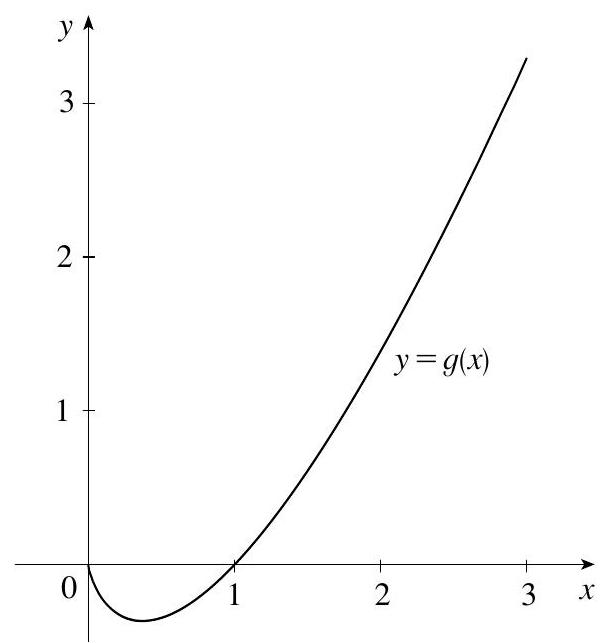
\includegraphics[max width=\textwidth, center]{2024_12_26_08a12fb3da5425a27925g-4}

It is a fact that the derivative of this function is $g^{\prime}(x)=\ln x+1$.

\begin{enumerate}
  \item Sketch the line tangent to $g(x)$ at $x=2$ on the graph above.
  \item Find an equation of the tangent line at $x=2$.
  \item Now sketch the line tangent to $g(x)$ at $x=\frac{1}{e} \approx 0.368$.
  \item Find an equation of the tangent line at $x=\frac{1}{e}$.
\end{enumerate}

\section*{GROUP WORK 3, SECTION 2.8}
\section*{The Derivative Function}
The graphs of several functions $f$ are shown below. For each function, estimate the slope of the graph of $f$ at various points. From your estimates, sketch graphs of $f^{\prime}$.\\
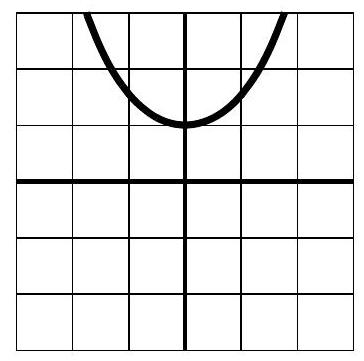
\includegraphics[max width=\textwidth, center]{2024_12_26_08a12fb3da5425a27925g-5(2)}

Graph 1\\
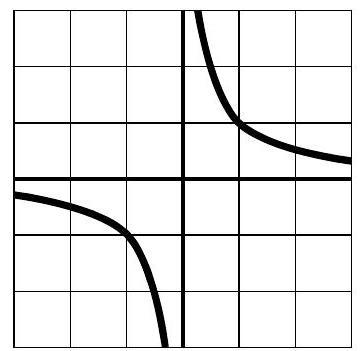
\includegraphics[max width=\textwidth, center]{2024_12_26_08a12fb3da5425a27925g-5}

Graph 3\\
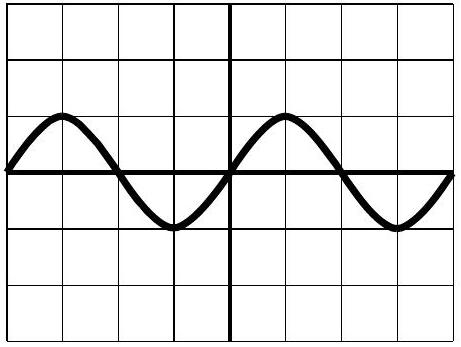
\includegraphics[max width=\textwidth, center]{2024_12_26_08a12fb3da5425a27925g-5(6)}

Graph 5\\
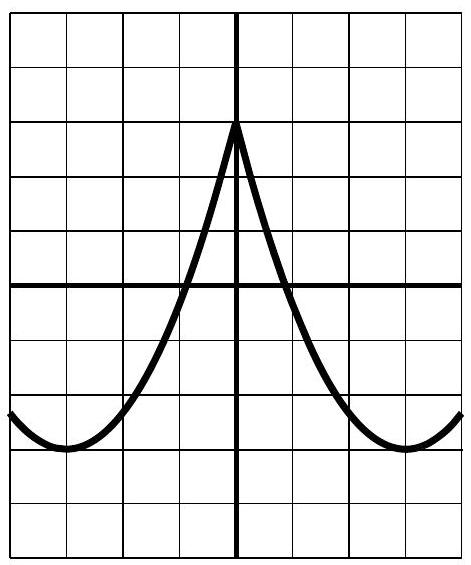
\includegraphics[max width=\textwidth, center]{2024_12_26_08a12fb3da5425a27925g-5(5)}

Graph 7\\
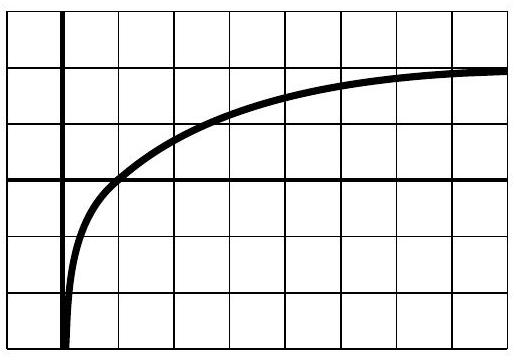
\includegraphics[max width=\textwidth, center]{2024_12_26_08a12fb3da5425a27925g-5(1)}

Graph 2\\
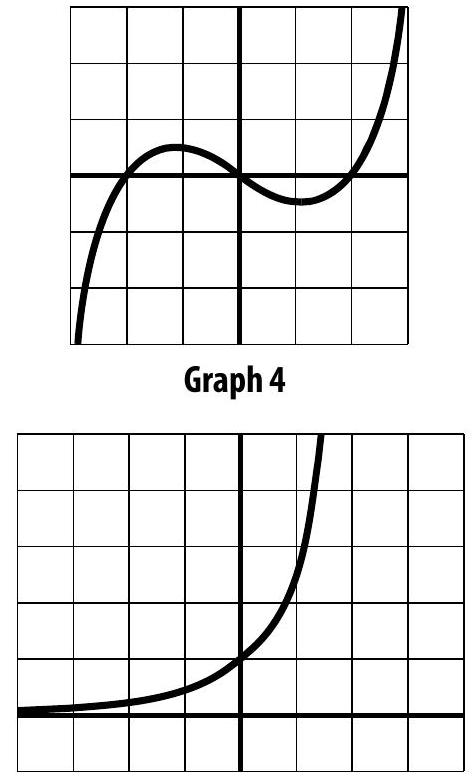
\includegraphics[max width=\textwidth, center]{2024_12_26_08a12fb3da5425a27925g-5(4)}

Graph 6\\
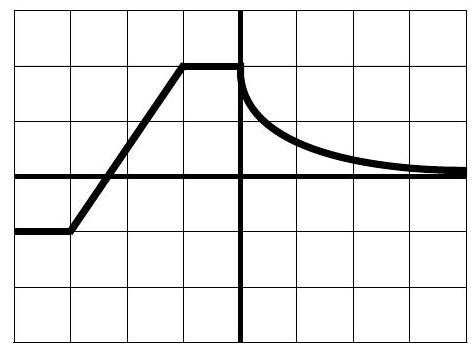
\includegraphics[max width=\textwidth, center]{2024_12_26_08a12fb3da5425a27925g-5(3)}

Graph 8


\end{document}